\chapter{अवक्षेपण और विलेयता}\label{ch:b1:precipitation}

सिल्वर नाइट्रेट की एक बूँद नल के पानी में गिरती है और एक सफ़ेद बादल दिखाई देता है:
सिल्वर क्लोराइड, जो हर लीटर में मौजूद कुछ मिलीग्राम क्लोराइड आयनों से बनता है।
चूना-पत्थर से रिसता पानी कैल्सियम कार्बोनेट को बहा ले जाता है और
उसे फिर से जमा करता है, साल में मिलीमीटर के एक अंश जितना, गुफा के
स्टैलेक्टाइटों के रूप में। गुर्दे की पथरी भी एक अवक्षेप है। इनमें से हर एक
किसी ठोस और विलयन में उसके आयनों के बीच का साम्य है, और एक
स्थिरांक, \omterm{def:b1:precipitation:solubility-product}{विलेयता गुणनफल}, बताता है कि ठोस बनता है या नहीं, उसका कितना
भाग घुलता है, और कोई दूसरा आयन मिलाने या pH बदलने पर उसकी \omterm{def:b1:precipitation:solubility}{विलेयता} कैसे
बदलती है। इसकी सहायता से रसायनज्ञ आयनों को एक-एक करके अवक्षेपित करके
उन्हें एक-दूसरे से अलग कर सकता है --- यही खदान के पानी के उपचार का
आधार है, जिससे यह अध्याय समाप्त होता है।

\begin{recall}
विद्यालय के खंड (कक्षा 6 और 12) ने \omterm{def:b1:precipitation:solubility}{विलेयता} को ग्राम प्रति
लीटर में मापा था और आयनों को उनके द्वारा दिए गए अवक्षेपों से पहचाना था। साम्य
स्थिरांक, \omterm{def:b1:extent-q-and-k:quotient}{अभिक्रिया भागफल} $Q$ और \omterm{def:b1:extent-q-and-k:activity}{सक्रियताएँ} (शुद्ध ठोस या विलायक के लिए 1,
विलेय के लिए $c/c^\circ$) \cref{ch:b1:extent-q-and-k} में स्थापित
की गईं: अभिक्रिया तब तक आगे बढ़ती है जब तक $Q < K$। प्रधान-अभिक्रिया विधि और
$\mathrm{p}K_a$ का पैमाना \cref{ch:b1:predominant-reaction} से आते हैं;
$c^\circ = \qty{1}{mol/L}$ भागफलों में नहीं
लिखा जाता।
\end{recall}

\begin{omfigure}
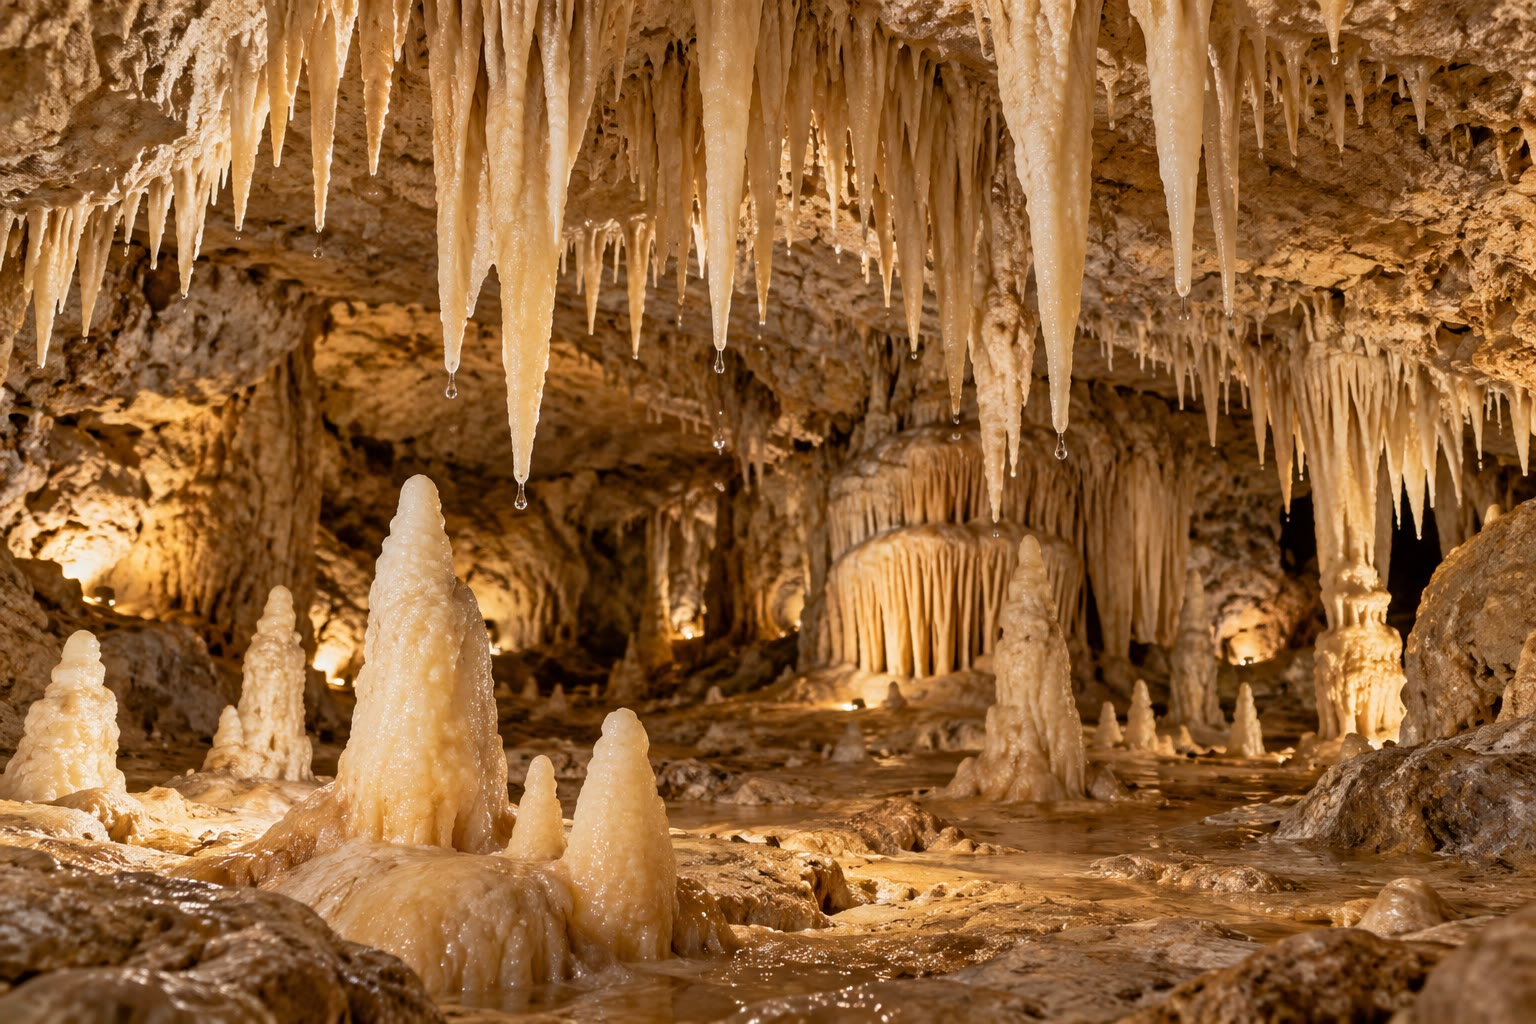
\includegraphics[width=0.62\linewidth]{images/book2/ai/b1-11-cave.jpg}

{\small चूना-पत्थर की गुफा में स्टैलेक्टाइट और स्टैलेग्माइट। कार्बन डाइऑक्साइड से
भरपूर पानी ऊपर की मिट्टी में कैल्सियम कार्बोनेट घोलता है; गुफा में
वह अपनी कुछ कार्बन डाइऑक्साइड खो देता है और कार्बोनेट फिर से अवक्षेपित होता है
(\cref{exo:b1:precipitation:10})।}
\end{omfigure}

\section{विलेयता गुणनफल}\label{sec:b1:precipitation:product}

पानी में डाला गया सिल्वर क्लोराइड का \omterm{def:b1:crystals-metals:crystal}{क्रिस्टल} विलयन को आयन देता है
और विलयन कुछ आयन \omterm{def:b1:crystals-metals:crystal}{क्रिस्टल} को लौटा देता है। जब दोनों
दरें बराबर हो जाती हैं, तो विलयन \emph{संतृप्त} होता है: उसका संघटन अब
नहीं बदलता, यद्यपि आयन दोनों दिशाओं में आते-जाते रहते हैं
(नीचे का चित्र)।

\begin{definition}[विलेयता गुणनफल]\label{def:b1:precipitation:solubility-product}
\emph{विलेयता गुणनफल}\index{विलेयता गुणनफल} $K_s$, किसी आयनिक ठोस
$\mathrm{M}_a\mathrm{X}_b$ के उसके आयनों में घुलने का साम्य स्थिरांक
है,
\[
  \mathrm{M}_a\mathrm{X}_b\mathrm{(s)} \rightleftharpoons a\,\mathrm{M}^{m+}
  + b\,\mathrm{X}^{x-}, \qquad
  K_s = [\mathrm{M}^{m+}]_{\mathrm{eq}}^{\,a}\,[\mathrm{X}^{x-}]_{\mathrm{eq}}^{\,b},
  \qquad \mathrm{p}K_s = -\log K_s ,
\]
जहाँ ठोस की \omterm{def:b1:extent-q-and-k:activity}{सक्रियता} 1 है। हर साम्य स्थिरांक की तरह यह
केवल ताप पर निर्भर करता है।
\end{definition}

सिल्वर क्लोराइड के लिए \ce{AgCl(s) <=> Ag+ + Cl-} और $K_s =
[\ce{Ag+}][\ce{Cl-}] = 10^{-9.75}$; कैल्सियम फ़्लुओराइड के लिए \ce{CaF2(s) <=>
Ca^2+ + 2F-} और $K_s = [\ce{Ca^2+}][\ce{F-}]^2 = 10^{-9.84}$;
आयरन(III) हाइड्रॉक्साइड के लिए $K_s = [\ce{Fe^3+}][\ce{OH-}]^3 = 10^{-38.55}$।
नीचे की सारणी इस खंड में प्रयुक्त मान देती है।
ये, \cref{ch:b1:predominant-reaction} के $\mathrm{p}K_a$ की तरह, सारणीबद्ध मानक
विरचन गिब्ज़ ऊर्जाओं से परिकलित हैं: $\mathrm{p}K_s = \Delta_r G^\circ/(RT\ln 10)$, एक संबंध
जो द्वितीय वर्ष के खंड में व्युत्पन्न किया गया है।

\begin{omfigure}
\begin{tikzpicture}[font=\small, >={Stealth}]
  % the crystal: alternating Ag+ (small, grey) and Cl- (large, green)
  \foreach \i in {0,1,2,3,4,5}
    \foreach \j in {0,1,2} {
      \pgfmathtruncatemacro{\pp}{mod(\i+\j,2)}
      \ifnum\pp=0
        \shade[ball color=green!55!black!60] (\i*0.62,\j*0.62) circle (0.29);
      \else
        \shade[ball color=gray!35] (\i*0.62,\j*0.62) circle (0.17);
      \fi }
  \draw[thick, gray] (-0.45,-0.45) rectangle (3.55,1.75);
  \node[below] at (1.55,-0.45) {\ce{AgCl(s)}};
  % ions in solution
  \shade[ball color=gray!35] (1.2,3.0) circle (0.17);
  \node[right] at (1.4,3.0) {\ce{Ag+}};
  \shade[ball color=green!55!black!60] (2.6,2.7) circle (0.29);
  \node[right] at (2.9,2.7) {\ce{Cl-}};
  \shade[ball color=gray!35] (4.4,1.4) circle (0.17);
  \shade[ball color=green!55!black!60] (5.1,2.6) circle (0.29);
  \shade[ball color=gray!35] (-1.0,2.4) circle (0.17);
  \shade[ball color=green!55!black!60] (-0.6,3.3) circle (0.29);
  % arrows: dissolution and precipitation
  \draw[->, thick, omDef] (1.24,1.6) to[bend left=20] node[left, pos=0.6] {घुलन} (1.15,2.78);
  \draw[->, thick, omProp] (2.55,2.38) to[bend left=20] node[right, pos=0.45] {अवक्षेपण} (2.45,1.55);
  % the water line
  \draw[blue!50, thick] (-1.6,3.8) -- (5.9,3.8);
  \node[blue!60!black, anchor=east] at (5.9,4.05) {संतृप्त विलयन};
\end{tikzpicture}

{\small अपने संतृप्त विलयन में सिल्वर क्लोराइड का एक \omterm{def:b1:crystals-metals:crystal}{क्रिस्टल}। आयन
सतह छोड़ते हैं (घुलन) और दूसरे आयन पकड़े जाते हैं (अवक्षेपण), एक ही
दर से, जिससे $[\ce{Ag+}][\ce{Cl-}]$, $K_s$ के बराबर बना रहता है। सिल्वर आयन
क्लोराइड आयनों से छोटे बनाए गए हैं, जैसे वे वास्तव में हैं।}
\end{omfigure}

\begin{omfigure}
\begin{tabular}{lc@{\qquad}lc}
\hline
ठोस & $\mathrm{p}K_s$ & ठोस & $\mathrm{p}K_s$ \\
\hline
\ce{AgCl} & 9.75 & \ce{Ca(OH)2} & 5.33 \\
\ce{AgBr} & 12.27 & \ce{Mg(OH)2} & 11.25 \\
\ce{AgI} & 16.07 & \ce{Fe(OH)2} & 16.31 \\
\ce{Ag2CrO4} & 11.95 & \ce{Zn(OH)2} & 16.38 \\
\ce{BaSO4} & 9.97 & \ce{Fe(OH)3} & 38.55 \\
\ce{CaCO3} (कैल्साइट) & 8.30 & \ce{Al(OH)3} (गिब्साइट) & 34.75 \\
\ce{CaF2} & 9.84 & & \\
\hline
\end{tabular}

\smallskip
{\small \qty{25}{\celsius} पर \omterm{def:b1:precipitation:solubility-product}{विलेयता गुणनफल}, ठोसों और जलीय
आयनों की मानक विरचन गिब्ज़ ऊर्जाओं से परिकलित। इस अध्याय में प्रयुक्त
विरचन स्थिरांक (\cref{sec:b1:precipitation:amphoteric}):
\ce{Zn(OH)4^2-} के लिए $\log\beta_4 = 14.45$, \ce{Al(OH)4-} के लिए 33.52, और
\ce{FeOH^2+} के लिए $\log\beta_1 = 11.82$।}
% ledger: dfg:AgCl_cr, dfg:AgBr_cr, dfg:AgI_cr, dfg:Ag2CrO4_cr, dfg:Ag+_ao, dfg:Cl-_ao, dfg:Br-_ao, dfg:I-_ao, dfg:CrO42-_ao (computed in figdata/bachelor-1/aqueous-constants.py)
% ledger: dfg:BaSO4_cr, dfg:Ba2+_ao, dfg:SO42-_ao, dfg:CaCO3_cr, dfg:CO32-_ao, dfg:CaF2_cr, dfg:Ca2+_ao, dfg:F-_ao (computed, same script)
% ledger: dfg:Ca_OH2_cr, dfg:Mg_OH2_cr, dfg:Mg2+_ao, dfg:Fe_OH2_cr, dfg:Fe2+_ao, dfg:Zn_OH2_cr, dfg:Zn2+_ao, dfg:Fe_OH3_cr, dfg:Fe3+_ao, dfg:Al2O3.3H2O_cr, dfg:Al3+_ao, dfg:OH-_ao (computed, same script)
% ledger: dfg:Zn_OH42-_ao, dfg:Al_OH4-_ao, dfg:FeOH2+_ao (formation constants, same script)
\end{omfigure}

\begin{proposition}[अवक्षेपण की शर्त]\label{prop:b1:precipitation:precipitation-condition}
मान लीजिए किसी विलयन में ठोस $\mathrm{M}_a\mathrm{X}_b$ के आयन हैं, और घुलन के लिए
\omterm{def:b1:extent-q-and-k:quotient}{अभिक्रिया भागफल} $Q_s = [\mathrm{M}^{m+}]^a[\mathrm{X}^{x-}]^b$ है।
\begin{itemize}
  \item यदि $Q_s < K_s$, तो ठोस साम्य पर उपस्थित नहीं रह सकता:
        विलयन असंतृप्त है और डाला गया कोई भी ठोस घुल जाता है, पूरी तरह,
        यदि वह बहुत अधिक न हो।
  \item यदि $Q_s > K_s$, तो ठोस तब तक अवक्षेपित होता है जब तक $Q_s = K_s$ न हो जाए।
  \item ठोस और विलयन साम्य पर केवल तभी साथ रहते हैं जब
        $Q_s = K_s$।
\end{itemize}
\end{proposition}

\begin{proof}
\cref{ch:b1:extent-q-and-k} के अनुसार घुलन तब तक आगे बढ़ता है जब तक
$Q_s < K_s$, और पीछे (अवक्षेपण) तब तक जब तक $Q_s > K_s$। जब
घुलन आगे बढ़ता है, $Q_s$ बढ़ता है। यदि ठोस
$Q_s$ के $K_s$ तक पहुँचने से पहले ही समाप्त हो जाए, तो विकास बिना किसी ठोस के रुक जाता है:
शुद्ध संघनित \omterm{def:b1:extent-q-and-k:system}{प्रावस्था} वाली अभिक्रिया साम्य से पहले रुक सकती है क्योंकि
उस \omterm{def:b1:extent-q-and-k:system}{प्रावस्था} की मात्रा ऋणात्मक नहीं हो सकती। यदि $Q_s > K_s$, तो अवक्षेपण
दोनों आयनों की सांद्रताएँ घटाता है और $Q_s$ तब तक घटता है जब तक $K_s$ के बराबर न हो जाए,
जो सदा संभव है, क्योंकि आयन उपस्थित हैं।
\end{proof}

अंतिम बिंदु ही ठोस को घुली हुई स्पीशीज़ से अलग करता है। कोई
अम्ल--क्षारक स्पीशीज़ हर pH पर उपस्थित होती है, चाहे कितनी भी कम; ठोस
या तो उपस्थित होता है या अनुपस्थित। इसीलिए उसका आरेख
\emph{अस्तित्व} आरेख होगा, \omterm{def:b1:predominant-reaction:predominance}{प्रभाविता आरेख} नहीं
(\cref{sec:b1:precipitation:domains})।

\begin{example}[दो विलयनों को मिलाना]\label{ex:b1:precipitation:mixing}
\qty{2.0e-4}{mol/L} सिल्वर नाइट्रेट के \qty{10.0}{mL} को
\qty{2.0e-4}{mol/L} सोडियम क्लोराइड के \qty{10.0}{mL} के साथ मिलाया जाता है। मिलाने के ठीक बाद,
किसी अभिक्रिया से पहले, $[\ce{Ag+}] = [\ce{Cl-}] = \qty{1.0e-4}{mol/L}$
और $Q_s = 10^{-8.0} > K_s = 10^{-9.75}$: सिल्वर क्लोराइड अवक्षेपित होता है।
दोनों विलयन \qty{2.0e-6}{mol/L} पर हों, तो $Q_s = 10^{-12.0} < K_s$ और
मिश्रण स्वच्छ रहता है। सिल्वर नाइट्रेट क्लोराइड आयनों का एक संवेदनशील परीक्षण है,
पर असीम रूप से संवेदनशील नहीं।
\end{example}

\begin{inthelab}[क्लोराइड परीक्षण]
शिक्षण प्रयोगशाला में नमूने को पहले तनु नाइट्रिक अम्ल से अम्लीय करके उसमें
सिल्वर नाइट्रेट विलयन की कुछ बूँदें डाली जाती हैं। अम्ल
कार्बोनेट और हाइड्रॉक्साइड आयनों को कार्बन डाइऑक्साइड और पानी में बदल देता है, जो
अन्यथा सिल्वर आयनों के साथ अवक्षेपित हो जाते। प्रकाश में काला पड़ने वाला
सफ़ेद अवक्षेप सिल्वर क्लोराइड है; ब्रोमाइड मलाई-रंग का अवक्षेप देता है
और आयोडाइड पीला
(नीचे का छायाचित्र)।
सिल्वर नाइट्रेट त्वचा पर काले धब्बे डालता है: दस्ताने और चश्मे पहने जाते हैं।
\end{inthelab}

\begin{omfigure}
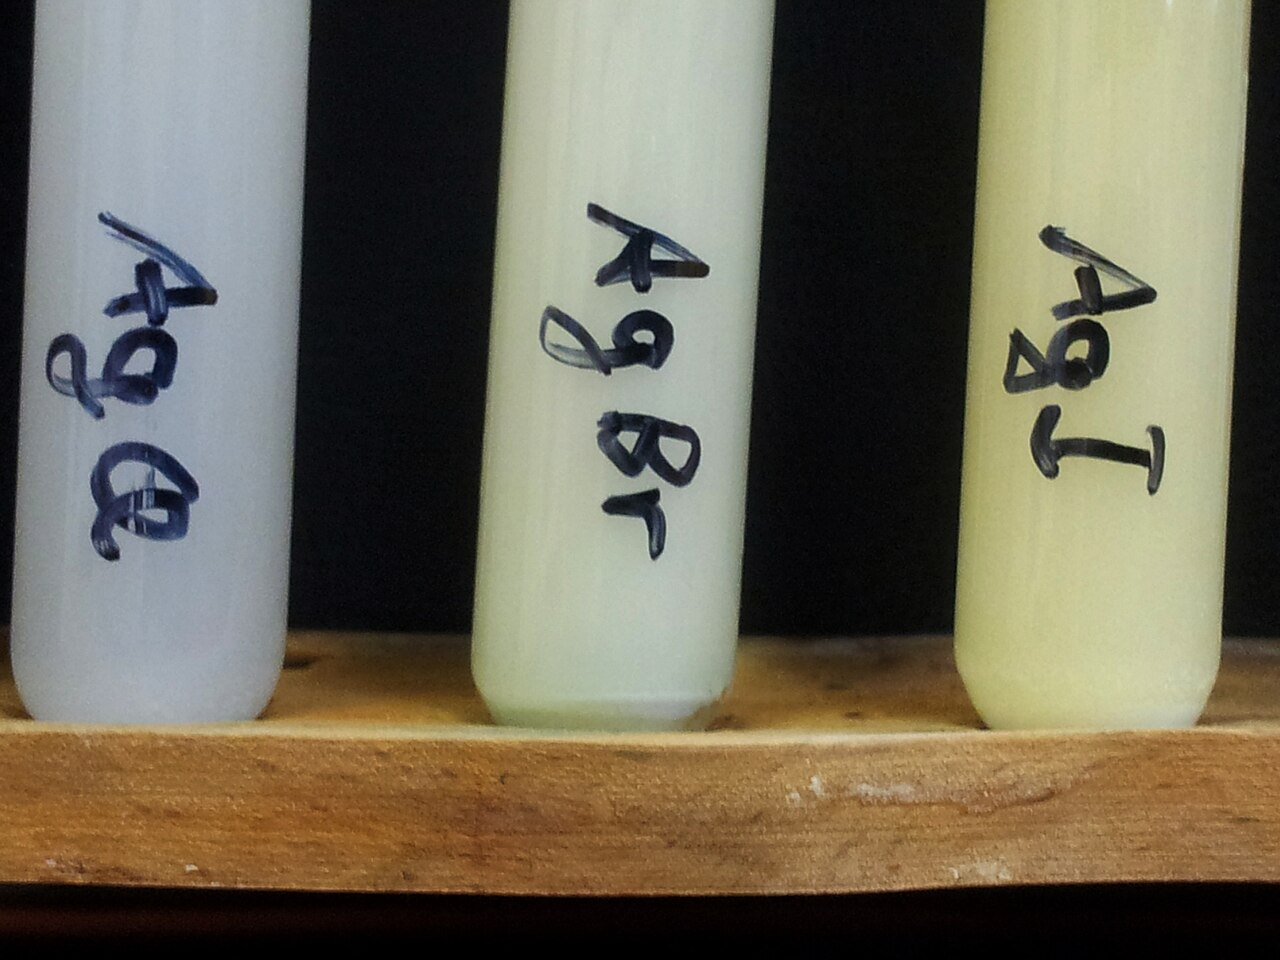
\includegraphics[width=0.6\linewidth]{images/book2/silver-halides.jpg}

{\small सिल्वर क्लोराइड (सफ़ेद), सिल्वर ब्रोमाइड (मलाई-रंग)
और सिल्वर आयोडाइड (हल्का पीला) के अवक्षेप। छायाचित्र: रराउश1974, CC BY-SA 3.0,
विकिमीडिया कॉमन्स।}
\end{omfigure}

\section{विलेयता}

\begin{definition}[विलेयता]\label{def:b1:precipitation:solubility}
किसी दिए गए विलयन में किसी ठोस की \emph{विलेयता}\index{विलेयता} $s$
ठोस की वह मात्रा है जो उस विलयन के एक लीटर में संतृप्ति तक
घुलती है (\unit{mol/L} में); मोलर द्रव्यमान से गुणा करने पर यह
द्रव्यमान विलेयता है, \unit{g/L} में। यह ताप पर और
विलयन के संघटन पर निर्भर करती है।
\end{definition}

\begin{proposition}[विलेयता गुणनफल से विलेयता]\label{prop:b1:precipitation:s-of-ks}
शुद्ध पानी में, यदि आयन किसी अन्य अभिक्रिया में भाग नहीं लेते,
\[
  \mathrm{MX}:\ s = \sqrt{K_s}, \qquad
  \mathrm{MX_2}\ \text{या}\ \mathrm{M_2X}:\ s = \left(\frac{K_s}{4}\right)^{1/3},
  \qquad
  \mathrm{M}_a\mathrm{X}_b:\ s = \left(\frac{K_s}{a^a b^b}\right)^{1/(a+b)} .
\]
\end{proposition}

\begin{proof}
जब प्रति लीटर $s$ mol ठोस घुलता है, तो $[\mathrm{M}^{m+}] = as$ और
$[\mathrm{X}^{x-}] = bs$, इसलिए संतृप्ति पर $K_s = (as)^a(bs)^b =
a^a b^b s^{a+b}$। MX के लिए $a = b = 1$; \ce{MX2} के लिए $1^1 2^2 = 4$, और
\ce{M2X} के लिए भी यही।
\end{proof}

\begin{example}[सिल्वर क्लोराइड और सिल्वर क्रोमेट]\label{ex:b1:precipitation:agcl-ag2cro4}
सिल्वर क्लोराइड: $s = 10^{-9.75/2} = \qty{1.3e-5}{mol/L}$, अर्थात्
$M = \qty{143.4}{g/mol}$ लेकर \qty{1.9}{mg/L}। सिल्वर क्रोमेट \ce{Ag2CrO4}
($\mathrm{p}K_s = 11.95$): $s = (10^{-11.95}/4)^{1/3} =
\qty{6.6e-5}{mol/L}$। क्रोमेट का $K_s$ छोटा है, फिर भी वह पाँच
गुना अधिक विलेय है। \omterm{def:b1:precipitation:solubility-product}{विलेयता गुणनफलों} की सीधी तुलना केवल
एक ही सूत्र-प्रकार के ठोसों के बीच की जा सकती है।
\end{example}

\begin{remark}
सूत्र मानते हैं कि आयन मुक्त हैं। शुद्ध पानी में क्रोमेट
आयन एक \omterm{def:b1:predominant-reaction:strong-acid}{दुर्बल क्षारक} है और सिल्वर आयन किसी से संकुलित नहीं होता, इसलिए
सिल्वर क्रोमेट का परिणाम लगभग सही है; किसी कार्बोनेट,
सल्फ़ाइड या हाइड्रॉक्साइड के लिए ऋणायन के क्षारकीय गुण मायने रखते हैं और
अगला खंड आवश्यक है। उच्च आयनिक सामर्थ्य पर \omterm{def:b1:extent-q-and-k:activity}{सक्रियताएँ} भी सांद्रताओं से
हट जाती हैं, एक संशोधन जो द्वितीय वर्ष के खंड पर छोड़ा गया है।
\end{remark}

\section{सम-आयन और pH प्रभाव}

\begin{definition}[सम-आयन प्रभाव]\label{def:b1:precipitation:common-ion}
\emph{सम-आयन प्रभाव}\index{सम-आयन प्रभाव} ऐसे विलयन में किसी ठोस की
\omterm{def:b1:precipitation:solubility}{विलेयता} का घटना है जिसमें उसका कोई आयन पहले से
मौजूद हो।
\end{definition}

\begin{proposition}[सम आयन के साथ विलेयता]\label{prop:b1:precipitation:common-ion}
मान लीजिए MX ऐसे विलयन में घुलता है जहाँ पहले से $[\mathrm{X}^-] = c$ है, और
$c \gg \sqrt{K_s}$। तब $s \approx K_s/c$, जो शुद्ध
पानी की तुलना में कहीं कम है। \ce{MX2} के लिए, ऐसे विलयन में जिसमें \ce{M^2+}, $c$ पर है,
$s \approx \frac12\sqrt{K_s/c}$।
\end{proposition}

\begin{proof}
संतृप्ति पर $[\mathrm{M}^+] = s$ और $[\mathrm{X}^-] = c + s$, इसलिए
$s(c + s) = K_s$। यदि $s \ll c$, तो $s = K_s/c$; यह मान्यता सही है क्योंकि
$K_s/c \ll c$, जब $c^2 \gg K_s$। \ce{MX2} के लिए $[\ce{X-}] = 2s$ और
$[\mathrm{M}^{2+}] = c + s \approx c$, इसलिए $c\,(2s)^2 = K_s$।
\end{proof}

\qty{0.10}{mol/L} सोडियम क्लोराइड में सिल्वर क्लोराइड: $s = 10^{-9.75}/0.10
= \qty{1.8e-9}{mol/L}$, पानी की तुलना में सात हज़ार गुना कम। इसीलिए
अवक्षेप को शुद्ध पानी के बजाय किसी सम आयन के तनु विलयन से धोया जाता है:
उसका कम भाग नष्ट होता है।

जब ठोस का ऋणायन क्षारक हो, तो अम्ल उसे घुलन-साम्य
से बाहर खींच लेता है और \omterm{def:b1:precipitation:solubility}{विलेयता} बढ़ जाती है। अम्ल में कैल्सियम कार्बोनेट के
लिए,
\[
  \ce{CaCO3(s) + H3O+ <=> Ca^2+ + HCO3- + H2O}, \qquad
  K = \frac{K_s}{K_{a2}} = 10^{-8.30 + 10.33} = 10^{2.03} ,
\]
जो एक अनुकूल अभिक्रिया है: सिरका या हाइड्रोक्लोरिक अम्ल चूना-पत्थर को घोल देता है,
और \ce{HCO3-} की आगे की अभिक्रिया से बनी कार्बन डाइऑक्साइड
परिचित झाग देती है।
% ledger: dfg:HCO3-_ao (pKa2 of carbonic acid, ch. 10)

\begin{proposition}[pH के सापेक्ष किसी हाइड्रॉक्साइड की विलेयता]\label{prop:b1:precipitation:hydroxide-ph}
किसी दिए गए pH पर बफ़र किए गए विलयन में \ce{M^{n+}} की वह सांद्रता, जो
हाइड्रॉक्साइड \ce{M(OH)_n} के साथ साम्य में है, इस संबंध का पालन करती है:
\[
  \log[\mathrm{M}^{n+}] = -\mathrm{p}K_s + n\,(\mathrm{p}K_e - \mathrm{pH}) ,
\]
जो pH के सापेक्ष प्रवणता $-n$ वाली सरल रेखा है। यदि आयन कोई संकुल नहीं बनाता,
तो यही हाइड्रॉक्साइड की \omterm{def:b1:precipitation:solubility}{विलेयता} है।
\end{proposition}

\begin{proof}
$K_s = [\mathrm{M}^{n+}][\ce{OH-}]^n$ और $[\ce{OH-}] = K_e/[\ce{H3O+}]$,
इसलिए $\log[\mathrm{M}^{n+}] = \log K_s - n\log[\ce{OH-}] = -\mathrm{p}K_s -
n(\mathrm{pH} - \mathrm{p}K_e)$।
\end{proof}

pH की हर इकाई आयरन(III) हाइड्रॉक्साइड की \omterm{def:b1:precipitation:solubility}{विलेयता} को एक
हज़ार से और ज़िंक हाइड्रॉक्साइड की \omterm{def:b1:precipitation:solubility}{विलेयता} को सौ से भाग कर देती है। हाइड्रॉक्साइडों को
pH बदलकर अवक्षेपित किया जाता है, और फिर से घोला जाता है।

\begin{example}[कार्बन डाइऑक्साइड से कैल्सियम कार्बोनेट घोलना]\label{ex:b1:precipitation:cave}
घुली हुई कार्बन डाइऑक्साइड वाला पानी कैल्साइट को घोलता है:
\[
  \ce{CaCO3(s) + CO2(aq) + H2O <=> Ca^2+ + 2HCO3-}, \qquad
  K = \frac{K_s K_{a1}}{K_{a2}} = 10^{-8.30 - 6.37 + 10.33} = 10^{-4.34} ,
\]
यह स्थिरांक कार्बोनेट के घुलन,
कार्बन डाइऑक्साइड की पहली अम्लता और दूसरी अम्लता की प्रतीप अभिक्रिया को जोड़कर प्राप्त होता है।
कार्बन डाइऑक्साइड जितनी अधिक, उतना अधिक कैल्सियम कार्बोनेट घुलता है। मिट्टी की वायु प्रायः
गुफा की वायु से कहीं अधिक कार्बन डाइऑक्साइड वाली होती है; जो पानी
मिट्टी पार करके गुफा की छत तक पहुँचता है वह कार्बन डाइऑक्साइड खो देता है, और
कैल्साइट जम जाता है (\cref{exo:b1:precipitation:10})।
\end{example}

\section{अस्तित्व क्षेत्र और वरणात्मक अवक्षेपण}\label{sec:b1:precipitation:domains}

\begin{definition}[अस्तित्व क्षेत्र]\label{def:b1:precipitation:existence-domain}
किसी ठोस और उसके किसी एक आयन की दी गई कुल सांद्रता $c$ के लिए, ठोस का
\emph{अस्तित्व क्षेत्र}\index{अस्तित्व क्षेत्र} चर (pX, pM या pH) का वह
परास है जिस पर ठोस साम्य पर उपस्थित रहता है। इसकी सीमा वह मान है जिस पर ठोस का
पहला कण प्रकट होता है, जब $Q_s = K_s$ और आयन अब भी सांद्रता $c$ पर हो।
\end{definition}

\begin{method}[अस्तित्व आरेख बनाना]\label{met:b1:precipitation:existence-domain}
\begin{enumerate}
  \item उस आयन की कुल सांद्रता $c$ तय कीजिए जो अक्ष पर नहीं है
        (उदाहरण के लिए pCl अक्ष पर $[\ce{Ag+}]_{\mathrm{tot}} = c$)।
  \item अवक्षेपण के आरंभ पर $K_s$ लिखिए, उस आयन को अब भी
        $c$ पर रखते हुए, और अक्ष के चर के लिए हल कीजिए।
  \item ठोस उस ओर अस्तित्व में होता है जहाँ दूसरा आयन
        सांद्र हो: छोटा pCl (बहुत क्लोराइड), छोटा pAg, या हाइड्रॉक्साइड के लिए
        ऊँचा pH।
  \item स्वयं आयन के लिए कोई क्षेत्र अंकित मत कीजिए: वह
        हर जगह उपस्थित है, ठोस के क्षेत्र के बाहर $c$ पर और उसके भीतर $c$ से
        नीचे।
\end{enumerate}
\end{method}

$c = [\ce{Ag+}]_{\mathrm{tot}} = 10^{-2}$ के साथ सिल्वर क्लोराइड के लिए:
अवक्षेपण तब आरंभ होता है जब $[\ce{Cl-}] = K_s/c = 10^{-7.75}$, इसलिए ठोस
$\mathrm{pCl} < 7.75$ के लिए अस्तित्व में होता है। सिल्वर आयोडाइड के लिए सीमा
$\mathrm{pI} = 16.07 - 2 = 14.07$ पर है, जैसा नीचे बनाया गया है।

\begin{omfigure}
\begin{tikzpicture}[font=\small, >={Stealth}, x=0.62cm]
  \fill[omDef!18] (0,0.12) rectangle (7.75,0.6);
  \draw[->, thick] (0,0) -- (17.2,0) node[right] {pCl या pI};
  \foreach \x in {0,2,4,6,8,10,12,14,16}
    \draw (\x,0.08) -- (\x,-0.08) node[below] {\x};
  \draw[omDef, thick] (7.75,-0.5) -- (7.75,0.9);
  \node[omDef] at (3.9,0.36) {\ce{AgCl(s)} उपस्थित};
  \node[omDef, above] at (7.75,0.9) {7.75};
  \node[anchor=west] at (8.0,0.36) {कोई ठोस नहीं: \ce{Ag+}, $10^{-2}$ mol/L पर};
  % AgI below
  \begin{scope}[yshift=-1.9cm]
  \fill[omProp!20] (0,0.12) rectangle (14.07,0.6);
  \draw[->, thick] (0,0) -- (17.2,0);
  \foreach \x in {0,2,4,6,8,10,12,14,16}
    \draw (\x,0.08) -- (\x,-0.08) node[below] {\x};
  \draw[omProp, thick] (14.07,-0.5) -- (14.07,0.9);
  \node[omProp] at (7.0,0.36) {\ce{AgI(s)} उपस्थित};
  \node[omProp, above] at (14.07,0.9) {14.07};
  \end{scope}
\end{tikzpicture}

{\small \qty{1.0e-2}{mol/L} की कुल सिल्वर सांद्रता के लिए सिल्वर क्लोराइड
(pCl अक्ष पर, ऊपर) और सिल्वर आयोडाइड (pI अक्ष पर, नीचे) के
\omterm{def:b1:precipitation:existence-domain}{अस्तित्व क्षेत्र}। आयोडाइड सिल्वर को क्लोराइड की तुलना में दस लाख
गुना कम सांद्रताओं पर अवक्षेपित कर देता है।}
\end{omfigure}

\begin{method}[वरणात्मक अवक्षेपण]\label{met:b1:precipitation:selective}
एक ही अभिकर्मक से अवक्षेपित होने वाले दो आयनों को अलग करने के लिए:
\begin{enumerate}
  \item हर आयन के लिए, उसकी अपनी सांद्रता पर, अभिकर्मक की वह
        सांद्रता (या pH) परिकलित कीजिए जिस पर उसका ठोस बनना शुरू होता है; जिसका
        मान कम हो, वह पहले अवक्षेपित होता है;
  \item जब दूसरा आयन अवक्षेपित होना शुरू हो, तब विलयन में बचे पहले आयन की
        सांद्रता परिकलित कीजिए;
  \item पृथक्करण स्वीकार्य है यदि वह सांद्रता प्रारंभिक सांद्रता का पर्याप्त
        छोटा भिन्न हो --- प्रायः \qty{0.1}{\percent}
        --- और तब अभिकर्मक को दोनों सीमाओं के बीच रोक दिया जाता है।
\end{enumerate}
\end{method}

\begin{example}[आयोडाइड और क्लोराइड]\label{ex:b1:precipitation:i-cl}
एक विलयन में आयोडाइड और क्लोराइड आयन हैं, दोनों
\qty{1.0e-2}{mol/L} पर; सिल्वर नाइट्रेट बूँद-बूँद, बिना
तनुकरण के, डाला जाता है। सिल्वर आयोडाइड $[\ce{Ag+}] = 10^{-16.07 + 2} =
10^{-14.07}$ पर बनना शुरू होता है, सिल्वर क्लोराइड $10^{-9.75 + 2} = 10^{-7.75}$ पर: आयोडाइड
पहले अवक्षेपित होता है। जब सिल्वर क्लोराइड प्रकट होता है, तब
$[\ce{I-}] = 10^{-16.07}/10^{-7.75} = 10^{-8.32} = \qty{4.8e-9}{mol/L}$,
जो आयोडाइड का $5 \times 10^{-7}$ भिन्न है: पृथक्करण पूर्ण है।
\end{example}

हाइड्रॉक्साइडों को इसी प्रकार pH को चर मानकर अलग किया जाता है।
नीचे का चार्ट \qty{0.010}{mol/L} पर छह आयनों के लिए
वह pH दिखाता है जहाँ हाइड्रॉक्साइड प्रकट होता है और वह pH जहाँ
आयन का \qty{99.9}{\percent} अवक्षेपित हो चुका होता है। आयरन(III) और ऐलुमिनियम
अम्लीय पानी में हट जाते हैं, ज़िंक और आयरन(II) उदासीनता के पास, मैग्नीशियम
pH 10 के आसपास और कैल्सियम केवल अत्यधिक क्षारकीय पानी में।

\begin{omfigure}
\begin{tikzpicture}
\begin{axis}[
  width=0.82\linewidth, height=5.4cm, xmin=0, xmax=14, ymin=0.4, ymax=6.6,
  axis x line=bottom, axis y line=left, xlabel={pH},
  xtick={0,2,4,6,8,10,12,14}, ytick={1,2,3,4,5,6},
  yticklabels={\ce{Fe^3+}, \ce{Al^3+}, \ce{Zn^2+}, \ce{Fe^2+}, \ce{Mg^2+}, \ce{Ca^2+}},
  y dir=reverse, axis line style={-},
  tick label style={font=\small}, label style={font=\small}]
\addplot[draw=none, omDef!35,
  error bars/.cd, x dir=plus, x explicit,
  error bar style={line width=7pt, omDef!35}, error mark=none]
  table[x=start, y=row, x error expr=14-\thisrow{start}] {figdata/out/bachelor-1-solubility-ph-thresholds.dat};
\addplot[draw=none, omDef,
  error bars/.cd, x dir=plus, x explicit,
  error bar style={line width=7pt, omDef}, error mark=none]
  table[x=start, y=row, x error expr=\thisrow{end}-\thisrow{start}] {figdata/out/bachelor-1-solubility-ph-thresholds.dat};
\end{axis}
\end{tikzpicture}

{\small हर आयन के \qty{0.010}{mol/L} वाले विलयनों से हाइड्रॉक्साइडों का
अवक्षेपण। गहरी पट्टी हाइड्रॉक्साइड के पहले कण से उस pH तक जाती है
जहाँ आयन का \qty{99.9}{\percent} अवक्षेपित हो चुका होता है (त्रिसंयोजी आयन के लिए
एक pH इकाई चौड़ी, द्विसंयोजी के लिए डेढ़); हल्की पट्टी हाइड्रॉक्साइड के
\omterm{def:b1:precipitation:existence-domain}{अस्तित्व क्षेत्र} का शेष भाग है। ऊँचे pH पर ज़िंक और ऐलुमिनियम हाइड्रॉक्साइडों का
उभयधर्मी पुनर्विलयन (\cref{sec:b1:precipitation:amphoteric}) नहीं दिखाया गया है।}
\end{omfigure}

\section{उभयधर्मी हाइड्रॉक्साइड}\label{sec:b1:precipitation:amphoteric}

ज़िंक सल्फ़ेट के विलयन में बूँद-बूँद सोडियम हाइड्रॉक्साइड डालिए: ज़िंक हाइड्रॉक्साइड का
सफ़ेद अवक्षेप बनता है, फिर आधिक्य हाइड्रॉक्साइड में वह फिर से घुल जाता है।
ऐलुमिनियम हाइड्रॉक्साइड भी ऐसा ही करता है; आयरन(III) और
मैग्नीशियम हाइड्रॉक्साइड नहीं।

\begin{definition}[उभयधर्मी हाइड्रॉक्साइड]\label{def:b1:precipitation:amphoteric-hydroxide}
कोई हाइड्रॉक्साइड \emph{उभयधर्मी हाइड्रॉक्साइड}\index{उभयधर्मी हाइड्रॉक्साइड} है
यदि वह अम्ल में धनायन के रूप में और आधिक्य क्षारक में
हाइड्रॉक्सो संकुल ऋणायन के रूप में, दोनों में घुलता है:
\[
  \ce{Zn(OH)2(s) + 2H3O+ -> Zn^2+ + 4H2O}, \qquad
  \ce{Zn(OH)2(s) + 2OH- -> Zn(OH)4^2-} .
\]
\end{definition}

संकुल ऋणायन \ce{Zn(OH)4^2-} (टेट्राहाइड्रॉक्सोज़िंकेट) को उसके
विरचन स्थिरांक द्वारा पहचाना जाता है, जिसका मान
$\beta_4 = [\ce{Zn(OH)4^2-}]/([\ce{Zn^2+}][\ce{OH-}]^4) = 10^{14.45}$ है; संकुल और उनके स्थिरांक
\cref{ch:b1:complexation} का विषय हैं।

\begin{proposition}[उभयधर्मी हाइड्रॉक्साइड की विलेयता]\label{prop:b1:precipitation:amphoteric}
यदि ज़िंक विलयन में केवल \ce{Zn^2+} और \ce{Zn(OH)4^2-} के रूप में है, तो
ज़िंक हाइड्रॉक्साइड की \omterm{def:b1:precipitation:solubility}{विलेयता} है
\[
  s = [\ce{Zn^2+}] + [\ce{Zn(OH)4^2-}] = \frac{K_s}{[\ce{OH-}]^2} + K\,[\ce{OH-}]^2,
  \qquad K = \beta_4 K_s = 10^{-1.93} .
\]
pH के सापेक्ष $\log s$ में यह निम्न pH पर प्रवणता $-2$ वाली रेखा का और
उच्च pH पर प्रवणता $+2$ वाली रेखा का अनुसरण करती है। यह न्यूनतम होती है
$[\ce{OH-}]^4 = K_s/K = 1/\beta_4$ पर, अर्थात् $\mathrm{pH} =
\mathrm{p}K_e - \frac14\log\beta_4$ पर, जहाँ $s_{\min} = 2\sqrt{K_s K}$।
\end{proposition}

\begin{proof}
संतृप्ति पर $[\ce{Zn^2+}] = K_s/[\ce{OH-}]^2$, और
$[\ce{Zn(OH)4^2-}] = \beta_4[\ce{Zn^2+}][\ce{OH-}]^4 = \beta_4 K_s
[\ce{OH-}]^2$। $w = [\ce{OH-}]^2$ के साथ $s(w) = K_s/w + Kw$ का अवकलज
$-K_s/w^2 + K$ है, जो $w = \sqrt{K_s/K}$ पर शून्य है, जहाँ $s = 2\sqrt{K_s K}$।
निम्न pH पर पहला पद प्रधान है और $\log s = \log K_s - 2\log[\ce{OH-}]$
(pH में प्रवणता $-2$); उच्च pH पर दूसरा, $\log s = \log K + 2\log[\ce{OH-}]$
(प्रवणता $+2$)।
\end{proof}

ऊपर के मानों से न्यूनतम $\mathrm{pH} = 14.00 - 14.45/4
= 10.39$ पर है और $s_{\min} = 2 \times 10^{-(16.38 + 1.93)/2} =
\qty{1.4e-9}{mol/L}$
(नीचे का चित्र)। वास्तविक
न्यूनतम कहीं ऊँचा है: ज़िंक \ce{ZnOH+}, \ce{Zn(OH)3-} और,
सबसे बढ़कर, एक अनावेशित घुला हुआ \ce{Zn(OH)2(aq)} भी बनाता है, जिसकी ठोस के साथ
साम्य में सांद्रता pH पर निर्भर नहीं करती। पूरा
परिकलन, उन्हीं सारणियों से, तल को लगभग
$10^{-5.6}$~mol/L पर रखता है। दो-स्पीशीज़ मॉडल प्रवणताएँ और
सीमाओं का क्रम देता है; न्यूनतम के पास हर स्पीशीज़ मायने रखती है।

\begin{omfigure}
\begin{tikzpicture}
\begin{axis}[name=zn,
  width=0.46\linewidth, height=5.6cm, xmin=6, xmax=14, ymin=-10, ymax=0,
  axis x line=bottom, axis y line=left, xlabel={pH}, ylabel={$\log s$},
  xtick={6,8,10,12,14}, ytick={-10,-8,-6,-4,-2,0},
  tick label style={font=\small}, label style={font=\small}]
\addplot[omProp, dashed, thick] table[x=pH, y=full] {figdata/out/bachelor-1-solubility-ph-zinc.dat};
\addplot[omDef, very thick] table[x=pH, y=model] {figdata/out/bachelor-1-solubility-ph-zinc.dat};
\node[font=\small, anchor=west] at (axis cs:7.0,-1.0) {\ce{Zn^2+}};
\node[font=\small, anchor=east] at (axis cs:13.8,-1.1) {\ce{Zn(OH)4^2-}};
\node[font=\small, omProp, anchor=south] at (axis cs:10.4,-5.5) {सभी स्पीशीज़};
\node[font=\small, anchor=north] at (axis cs:10.2,-0.4) {ज़िंक};
\end{axis}
\begin{axis}[at={(zn.east)}, anchor=west, xshift=1.8cm,
  width=0.46\linewidth, height=5.6cm, xmin=2, xmax=14, ymin=-10, ymax=0,
  axis x line=bottom, axis y line=left, xlabel={pH}, ylabel={$\log s$},
  xtick={2,4,6,8,10,12,14}, ytick={-10,-8,-6,-4,-2,0},
  tick label style={font=\small}, label style={font=\small}]
\addplot[omDef, very thick] table[x=pH, y=model] {figdata/out/bachelor-1-solubility-ph-aluminium.dat};
\node[font=\small, anchor=west] at (axis cs:3.4,-0.8) {\ce{Al^3+}};
\node[font=\small, anchor=east] at (axis cs:13.8,-0.6) {\ce{Al(OH)4-}};
\node[font=\small, anchor=north] at (axis cs:8.6,-0.4) {ऐलुमिनियम};
\end{axis}
\end{tikzpicture}

{\small pH के सापेक्ष ज़िंक हाइड्रॉक्साइड (बाएँ) और ऐलुमिनियम हाइड्रॉक्साइड,
गिब्साइट (दाएँ), की \omterm{def:b1:precipitation:solubility}{विलेयता}, दो-स्पीशीज़ मॉडल (ठोस रेखाएँ): प्रवणताएँ
ज़िंक के लिए $-2$ और $+2$, ऐलुमिनियम के लिए $-3$ और $+1$। ज़िंक के लिए डैश वक्र में सभी
हाइड्रॉक्सो स्पीशीज़ शामिल हैं, और अनावेशित \ce{Zn(OH)2(aq)} एक तल निर्धारित करता है।}
\end{omfigure}

ऐलुमिनियम के लिए हाइड्रॉक्साइड \ce{Al(OH)3} है और संकुल \ce{Al(OH)4-},
इसलिए अभिक्रिया $\ce{Al(OH)3(s) + OH- <=> Al(OH)4-}$ है, जिसका स्थिरांक
$K = \beta_4 K_s = 10^{33.52 - 34.75} = 10^{-1.23}$ है, और प्रवणताएँ $-3$ और $+1$ हैं। ऐलुमिनियम और
आयरन(III) का अंतर --- एक उभयधर्मी, दूसरा नहीं --- उद्योग में उन्हें
अलग करने के लिए प्रयुक्त होता है: गर्म सोडियम हाइड्रॉक्साइड बॉक्साइट के
ऐलुमिनियम को घोल लेता है और आयरन ऑक्साइडों को पीछे छोड़ देता है
(\cref{exo:b1:precipitation:12})।

\section{अभ्यास}

\begin{exercise}[$\star$]\label{exo:b1:precipitation:1}
\ce{BaSO4}, \ce{CaF2}, \ce{Ag2CrO4} और \ce{Fe(OH)3} के लिए घुलन का समीकरण और
$K_s$ का व्यंजक लिखिए। \cref{sec:b1:precipitation:product} की सारणी से $K_s$ दस की घातों में
बताइए, और उस ठोस का $\mathrm{p}K_s$ भी जिसका $K_s = \num{2.0e-13}$ है।
\end{exercise}

\begin{exercise}[$\star$]\label{exo:b1:precipitation:2}
शुद्ध पानी में सिल्वर ब्रोमाइड की \omterm{def:b1:precipitation:solubility}{विलेयता} \unit{mol/L} में
और \unit{mg/L} में परिकलित कीजिए ($M = \qty{187.8}{g/mol}$)।
\end{exercise}

\begin{exercise}[$\star$]\label{exo:b1:precipitation:3}
\qty{2.0e-3}{mol/L} बेरियम क्लोराइड के \qty{50}{mL} को
\qty{2.0e-4}{mol/L} सोडियम सल्फ़ेट के \qty{50}{mL} के साथ मिलाया जाता है। क्या बेरियम
सल्फ़ेट अवक्षेपित होता है? यही प्रश्न, सोडियम सल्फ़ेट
\qty{2.0e-7}{mol/L} पर हो तो।
\end{exercise}

\begin{exercise}[$\star$]\label{exo:b1:precipitation:4}
शुद्ध पानी में बेरियम सल्फ़ेट की \omterm{def:b1:precipitation:solubility}{विलेयता} परिकलित कीजिए, फिर
\qty{0.010}{mol/L} सोडियम सल्फ़ेट विलयन में। यह कितने गुना
बदली है?
\end{exercise}

\begin{exercise}[$\star\star$]\label{exo:b1:precipitation:5}
शुद्ध पानी में कैल्सियम फ़्लुओराइड की \omterm{def:b1:precipitation:solubility}{विलेयता} (\unit{mol/L} और
\unit{mg/L}, $M = \qty{78.1}{g/mol}$) परिकलित कीजिए, फिर \qty{0.10}{mol/L}
कैल्सियम क्लोराइड विलयन में। अपने किए गए सन्निकटन की जाँच कीजिए।
\end{exercise}

\begin{exercise}[$\star\star$]\label{exo:b1:precipitation:6}
एक विलयन में \qty{0.050}{mol/L} मैग्नीशियम आयन हैं। किस pH पर
मैग्नीशियम हाइड्रॉक्साइड अवक्षेपित होना शुरू होता है? किस pH पर
मैग्नीशियम का \qty{99}{\percent} अवक्षेपित हो चुका होता है? pH अक्ष पर \ce{Mg(OH)2} का
\omterm{def:b1:precipitation:existence-domain}{अस्तित्व क्षेत्र} बनाइए।
\end{exercise}

\begin{exercise}[$\star\star$]\label{exo:b1:precipitation:7}
एक विलयन में ब्रोमाइड और क्लोराइड आयन हैं, दोनों
\qty{1.0e-2}{mol/L} पर। सिल्वर नाइट्रेट बिना तनुकरण के डाला जाता है। कौन-सा
अवक्षेप पहले प्रकट होता है? जब दूसरा ठोस प्रकट होता है, तब पहले आयन का कितना भिन्न
अब भी विलयन में है? क्या पृथक्करण स्वीकार्य है?
\end{exercise}

\begin{exercise}[$\star\star$]\label{exo:b1:precipitation:8}
सिल्वर आयनों द्वारा क्लोराइड का मोर अनुमापन क्रोमेट आयनों को
सूचक के रूप में प्रयुक्त करता है: लाल सिल्वर क्रोमेट तभी प्रकट होना चाहिए जब लगभग सारा
क्लोराइड अवक्षेपित हो चुका हो। क्लोराइड \qty{0.050}{mol/L} पर है और क्रोमेट
\qty{5.0e-3}{mol/L} पर; तनुकरण नगण्य माना गया है। जब सिल्वर क्रोमेट बनना
शुरू होता है, तब $[\ce{Ag+}]$ परिकलित कीजिए, और उस क्षण विलयन में बचे
क्लोराइड का भिन्न भी।
\end{exercise}

\begin{exercise}[$\star\star$]\label{exo:b1:precipitation:9}
कैल्सियम कार्बोनेट को ऐसे विलयन के साथ हिलाया जाता है जिसे एक बफ़र pH 8.30 पर रखता है,
जहाँ हाइड्रोजनकार्बोनेट कार्बोनेट की कहीं प्रमुख स्पीशीज़ है। दिखाइए कि
$[\ce{Ca^2+}][\ce{HCO3-}] = K_s\,10^{\mathrm{p}K_{a2} - \mathrm{pH}}$, और
यह मानकर कि घुला सारा कार्बोनेट
\ce{HCO3-} के रूप में रहता है ($\mathrm{p}K_{a2} = 10.33$), \omterm{def:b1:precipitation:solubility}{विलेयता} परिकलित कीजिए।
\end{exercise}

\begin{exercise}[$\star\star\star$]\label{exo:b1:precipitation:10}
चूना-पत्थर की गुफाएँ। कार्बन डाइऑक्साइड की \omterm{def:b1:precipitation:solubility}{विलेयता}
\ce{CO2(g) <=> CO2(aq)} का पालन करती है, $\log K_H = -1.47$ के साथ ($K_H =
[\ce{CO2(aq)}]/p(\ce{CO2})$, दाब बार में)।
\begin{enumerate}
  \item $K_H$ को \cref{ex:b1:precipitation:cave} के स्थिरांक के साथ
        मिलाकर
        \ce{CaCO3(s) + CO2(g) + H2O <=> Ca^2+ + 2HCO3-} का स्थिरांक प्राप्त कीजिए।
  \item दिखाइए कि कैल्साइट की \omterm{def:b1:precipitation:solubility}{विलेयता} $s = (K'p/4)^{1/3}$ है और
        उसे उस पानी में परिकलित कीजिए जो मिट्टी की वायु के साथ साम्य में आ चुका है,
        $p(\ce{CO2}) = \qty{0.010}{bar}$, फिर बाहरी वायु के साथ,
        \qty{4.26e-4}{bar}। दोनों को \ce{CaCO3} के \unit{mg/L} में दीजिए
        ($M = \qty{100.1}{g/mol}$)।
  \item स्टैलेक्टाइट की वृद्धि समझाइए।
\end{enumerate}
\end{exercise}

\begin{exercise}[$\star\star\star$]\label{exo:b1:precipitation:11}
\qty{1.0e-2}{mol/L} ज़िंक के एक विलयन को बढ़ते pH पर लाया जाता है,
और ज़िंक केवल \ce{Zn^2+} और \ce{Zn(OH)4^2-} के रूप में उपस्थित है।
\begin{enumerate}
  \item किन pH मानों के बीच ज़िंक हाइड्रॉक्साइड उपस्थित है?
  \item न्यूनतम \omterm{def:b1:precipitation:solubility}{विलेयता} का pH और न्यूनतम \omterm{def:b1:precipitation:solubility}{विलेयता} ज्ञात कीजिए।
  \item pH के सापेक्ष $\log s$ का रेखाचित्र बनाइए और प्रवणताएँ अंकित कीजिए।
\end{enumerate}
\end{exercise}

\begin{exercise}[$\star\star\star$]\label{exo:b1:precipitation:12}
एक विलयन में ऐलुमिनियम और आयरन(III) आयन हैं, हर एक
\qty{1.0e-3}{mol/L} पर। सोडियम हाइड्रॉक्साइड आधिक्य में डाला जाता है।
\begin{enumerate}
  \item किस pH से ऊपर सारा ऐलुमिनियम \ce{Al(OH)4-} के रूप में घुल जाता है?
  \item तब \ce{Fe^3+} की सांद्रता क्या है? पृथक्करण के बारे में
        निष्कर्ष निकालिए।
  \item समझाइए कि ऐलुमिनियम के स्थान पर मैग्नीशियम होने पर पृथक्करण क्यों
        विफल होता।
\end{enumerate}
\end{exercise}

\section{समस्या: खदान के बहिःस्राव की सफ़ाई}

\begin{problem}[{सप्ताहांत समस्या --- तीन हाइड्रॉक्साइडों की अवक्षेपण-सीमाएँ,
आयरन(III) का हाइड्रॉक्सो संकुल, ज़िंक की पुनःप्राप्ति और
उसका उभयधर्मी पुनर्विलयन, और ज़िंक(II) खोए बिना आयरन(III) हटाने की pH खिड़की}]
\label{pb:b1:precipitation:1}
किसी पुरानी धातु-खदान से निकलने वाला पानी अम्लीय (pH 2.0) है और उसमें
\qty{1.0e-3}{mol/L} आयरन(III), \qty{5.0e-3}{mol/L} ज़िंक(II) और
\qty{2.0e-2}{mol/L} मैग्नीशियम है। संयंत्र pH को चरणबद्ध बढ़ाता है ताकि
आयरन अपशिष्ट गाद के रूप में हट जाए, फिर ज़िंक उसके
हाइड्रॉक्साइड के रूप में पुनःप्राप्त हो, और हानिरहित मैग्नीशियम पानी में रह जाए।
\qty{25}{\celsius} पर आँकड़े: $\mathrm{p}K_s$: \ce{Fe(OH)3} 38.55, \ce{Zn(OH)2}
16.38, \ce{Mg(OH)2} 11.25; $\log\beta_4(\ce{Zn(OH)4^2-}) = 14.45$;
$\log\beta_1(\ce{FeOH^2+}) = 11.82$; $\mathrm{p}K_e = 14.00$; मोलर द्रव्यमान
\ce{Fe(OH)3} \qty{106.8}{g/mol}, \ce{Zn(OH)2} \qty{99.4}{g/mol}।

\medskip
\noindent\textbf{भाग I --- पहले कौन-सा हाइड्रॉक्साइड?}
\begin{enumerate}
  \item तीनों हाइड्रॉक्साइडों के घुलन-साम्य और
        उनके $K_s$ लिखिए।
  \item समझाइए कि केवल तीन $\mathrm{p}K_s$ यह क्यों नहीं बताते कि कौन-सा
        हाइड्रॉक्साइड पहले अवक्षेपित होता है।
  \item दिखाइए कि \ce{M(OH)_n}, $c$ पर \ce{M^{n+}} वाले विलयन से,
        $\mathrm{pH} = \mathrm{p}K_e -
        \frac1n(\mathrm{p}K_s + \log c)$ पर अवक्षेपित होना शुरू होता है।
  \item आयरन(III) के लिए यह pH परिकलित कीजिए।
  \item ज़िंक के लिए परिकलित कीजिए।
  \item मैग्नीशियम के लिए परिकलित कीजिए।
  \item pH बढ़ने के साथ अवक्षेपण का क्रम बताइए। क्या खदान से निकलते समय
        बहिःस्राव में कुछ अवक्षेपित होता है?
\end{enumerate}

\medskip
\noindent\textbf{भाग II --- आयरन हटाना: पहला अनुमान।}
\begin{enumerate}[resume]
  \item संयंत्र पानी से आयरन का \qty{99.9}{\percent} निकालना चाहता है। इससे
        घुले हुए आयरन की कितनी सांद्रता अनुमत होती है?
  \item किसी संकुल को नगण्य मानकर, यह किस pH पर प्राप्त होती है?
  \item दिखाइए कि \ce{Fe(OH)3} के \omterm{def:b1:precipitation:existence-domain}{अस्तित्व क्षेत्र} में
        $\log[\ce{Fe^3+}]$ प्रति pH इकाई 3 घटता है।
  \item किस pH तक ज़िंक पूरी तरह विलयन में रहता है?
  \item उस pH खिड़की का पहला अनुमान दीजिए जिसमें आयरन हट जाता है
        जबकि ज़िंक रहता है।
\end{enumerate}

\medskip
\noindent\textbf{भाग III --- आयरन(III) का हाइड्रॉक्सो संकुल।}
\begin{enumerate}[resume]
  \item \ce{FeOH^2+} का विरचन लिखिए, \ce{Fe^3+} और \ce{OH-} से,
        और उसका स्थिरांक।
  \item pH के सापेक्ष \ce{Fe^3+} और \ce{FeOH^2+} का \omterm{def:b1:predominant-reaction:predominance}{प्रभाविता आरेख}
        बनाइए।
  \item प्रश्न 9 में प्राप्त pH पर
        $[\ce{FeOH^2+}]/[\ce{Fe^3+}]$ परिकलित कीजिए। क्या पहला अनुमान सुरक्षित था?
  \item कुल घुले आयरन $[\ce{Fe^3+}] + [\ce{FeOH^2+}]$ को, जो
        \ce{Fe(OH)3} के साथ साम्य में है, pH के फलन के रूप में व्यक्त कीजिए।
  \item दिखाइए कि जहाँ \ce{FeOH^2+} प्रभावी है, वहाँ उसका लघुगणक
        प्रति pH इकाई 2 घटता है।
  \item वह pH ज्ञात कीजिए जिस पर कुल घुला आयरन प्रश्न 8 के
        मान तक गिर जाता है।
\end{enumerate}

\medskip
\noindent\textbf{भाग IV --- ज़िंक की पुनःप्राप्ति।}
\begin{enumerate}[resume]
  \item आयरन की गाद छान लेने के बाद pH फिर बढ़ाया जाता है। किस
        pH पर ज़िंक का \qty{99}{\percent} अवक्षेपित हो जाता है? क्या उस pH पर मैग्नीशियम
        हाइड्रॉक्साइड बनता है?
  \item ज़िंक हाइड्रॉक्साइड की आधिक्य हाइड्रॉक्साइड आयनों के साथ अभिक्रिया लिखिए
        और उसका स्थिरांक परिकलित कीजिए।
  \item किस pH से ऊपर सारा ज़िंक फिर से विलयन में होगा? संचालक के लिए
        इसका क्या अर्थ है?
  \item प्रति घन मीटर बहिःस्राव से हटाई गई आयरन(III) हाइड्रॉक्साइड गाद का
        द्रव्यमान परिकलित कीजिए।
  \item प्रश्न 19 के pH पर प्रति घन मीटर पुनःप्राप्त ज़िंक हाइड्रॉक्साइड का
        द्रव्यमान परिकलित कीजिए।
  \item आयरन को ज़िंक से पहले क्यों हटाना चाहिए, दोनों को
        एक साथ क्यों नहीं?
  \item दो दशमलव स्थानों तक वह pH खिड़की बताइए जिसमें आयरन(III)
        \qty{99.9}{\percent} तक हट जाता है जबकि ज़िंक(II) पूरी तरह
        विलयन में रहता है।
\end{enumerate}
\end{problem}
